\documentclass[tikz,border=2pt,11pt]{standalone}
\usetikzlibrary{arrows.meta}
\usetikzlibrary{decorations.pathreplacing}
\usetikzlibrary{positioning}
\usetikzlibrary{calc}
\usepackage{amsmath}
\usepackage{amssymb}
\usepackage{graphicx}
\usepackage{xcolor}
\usepackage{tikz}
\newcommand{\R}{\mathbb R}
\newcommand{\Z}{\mathbb Z}
\newcommand{\N}{\mathbb N}
\newcommand{\F}{\mathbb F}
\newcommand{\E}{\mathbb E}
\newcommand{\Pp}{\mathbb P}
\newcommand{\one}{\mathbf 1}
\newcommand{\Id}{\mathrm{Id}}
\DeclareMathOperator{\TV}{TV}
\DeclareMathOperator{\supp}{supp}
\DeclareMathOperator{\rank}{rank}
\DeclareMathOperator{\diag}{diag}
\DeclareMathOperator{\Span}{span}
\DeclareMathOperator{\KL}{D}
\DeclareMathOperator{\dist}{dist}
\DeclareMathOperator{\diam}{diam}
\DeclareMathOperator{\Lip}{Lip}
\DeclareMathOperator{\tr}{tr}
\DeclareMathOperator{\osc}{osc}
\newcommand{\ip}[2]{\langle #1,#2\rangle}
\begin{document}
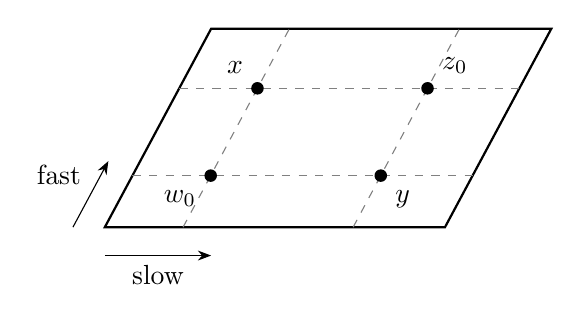
\begin{tikzpicture}[x=.9cm,y=.9cm,>=Stealth,
 point/.style={circle,fill,inner sep=1.6pt}]
 \draw[thick] (0,0)--(4.8,0)--(6.3,2.8)--(1.5,2.8)--cycle;
 \draw[dashed,gray] (1.104,0)--(2.604,2.8);
 \draw[dashed,gray] (3.504,0)--(5.004,2.8);
 \draw[dashed,gray] (.39,.728)--(5.19,.728);
 \draw[dashed,gray] (1.05,1.96)--(5.85,1.96);
 \node[point,label=above left:{$x$}] at (2.154,1.96) {};
 \node[point,label=below right:{$y$}] at (3.894,.728) {};
 \node[point,label=above right:{$z_0$}] at (4.554,1.96) {};
 \node[point,label=below left:{$w_0$}] at (1.494,.728) {};
 \draw[->] (0,-.4)--(1.5,-.4) node[midway,below] {slow};
 \draw[->] (-.45,0)--(.05,.933) node[midway,above left] {fast};
\end{tikzpicture}
\end{document}
